\section{Phương pháp và kiến trúc nghiên cứu}
\label{sec:methodology}

%------------------------------------------------------------------------------
\subsection{Tổng quan phương pháp}
\label{subsec:methodology_overview}

Nghiên cứu này giải quyết bài toán dự báo phụ tải điện theo giờ trên tập dữ liệu PG\&E gồm ba năm (2020--2022) với các biến ngoại sinh nhiệt độ và bức xạ mặt trời thu thập từ 5 trạm quan trắc địa lý. Chúng tôi đề xuất kiến trúc \textbf{Context-Aware Stacking (CAS)}, một phương pháp học kết hợp hai tầng tích hợp các đặc trưng vật lý nhằm khắc phục các hạn chế của mô hình cơ sở đơn lẻ trước đó.

Chiến lược nghiên cứu được tổ chức thành bốn mô-đun liên hoàn, được minh họa tổng thể trong Hình~\ref{fig:methodology_architecture}: (i)~\textbf{Mô-đun~1} giải quyết đa cộng tuyến ngoại sinh bằng PCA; (ii)~\textbf{Mô-đun~2} bổ sung đặc trưng vật lý về nhu cầu nhiệt (CDD/HDD) và sóng Fourier liên tục; (iii)~\textbf{Mô-đun~3} phân tích tính bù trừ sai số giữa hai chế độ vận hành (ngày và đêm) để lựa chọn mô hình cơ sở phù hợp; (iv)~\textbf{Mô-đun~4} xây dựng mô hình kết hợp theo ngữ cảnh CAS.

\begin{figure}[htbp]
    \centering
    \begin{tcolorbox}[colback=gray!5,colframe=aivnGreen,arc=3mm,boxrule=0.8pt,width=0.98\linewidth,title={\bfseries Khung kiến trúc tổng thể: Context-Aware Stacking (CAS)},fonttitle=\sffamily\bfseries]
    \centering
    \small
    \begin{verbatim}
┌────────────────────────────────────────────────────────────────────────────────────────┐
│                              DỮ LIỆU ĐẦU VÀO NGOẠI SINH                                │
│    5 Trạm Quan trắc Nhiệt độ (T1..T5)      5 Trạm Quan trắc Bức xạ Mặt trời (G1..G5)   │
└───────────────────────────┬────────────────────────────────┬───────────────────────────┘
                            │                                │
                 ┌──────────▼──────────┐          ┌──────────▼──────────┐
                 │  PCA Giảm Chiều Temp│          │  PCA Giảm Chiều GHI │
                 │     (VIF: 48 -> 2.4)│          │   (VIF: 1055 -> 2.0)│
                 └──────────┬──────────┘          └──────────┬──────────┘
                            │                                │
                            ▼                                ▼
┌────────────────────────────────────────────────────────────────────────────────────────┐
│                        KỸ THUẬT TRÍCH XUẤT ĐẶC TRƯNG VẬT LÝ                            │
│   • Nhu cầu nhiệt: Heating / Cooling Degree Days (HDD & CDD tại ngưỡng cơ sở 18°C)     │
│   • Chu kỳ Sóng Fourier liên tục: Sin/Cos(DOY / 365.25) & Sin/Cos(Hour / 24)           │
│   • Biến động học trễ thời gian: PCA_Temp_Lag1, PCA_GHI_Lag1                           │
└───────────────────────────┬────────────────────────────────┬───────────────────────────┘
                            │                                │
                 ┌──────────▼──────────┐          ┌──────────▼──────────┐
                 │   Mô hình Cơ sở 1   │          │   Mô hình Cơ sở 2   │
                 │  ElasticNet (Tuyến  │          │   XGBoost (Phi tuyến│
                 │   tính, Phụ tải nền)│          │    Cây, Phụ tải đỉnh│
                 └──────────┬──────────┘          └──────────┬──────────┘
                            │ ŷ_linear                       │ ŷ_tree
                            └───────────────┬────────────────┘
                                            │
                                            ▼
┌────────────────────────────────────────────────────────────────────────────────────────┐
│                   MÔ HÌNH TỔNG HỢP THEO NGỮ CẢNH (LIGHTGBM - CAS)                      │
│   Vector Đầu vào Ghép nối: [ŷ_linear, ŷ_tree]  +  [Hour, HDD, CDD, Fourier, Weather]   │
│   • Ban đêm (00:00 - 06:00): Tự động ưu tiên trọng số dự báo của ElasticNet            │
│   • Sóng nhiệt (CDD > 3°C) : Tự động tăng tỷ trọng cho XGBoost                         │
└───────────────────────────────────────────┬────────────────────────────────────────────┘
                                            │
                                            ▼
                                   DỰ BÁO PHỤ TẢI CUỐI CÙNG
    \end{verbatim}
    \end{tcolorbox}
    \caption{Khung phương pháp Context-Aware Stacking (CAS) tích hợp đặc trưng vật lý.}
    \label{fig:methodology_architecture}
\end{figure}

%------------------------------------------------------------------------------
\subsection{Phương pháp cơ sở đối chuẩn (Baseline Method)}
\label{subsec:baseline}

Phương pháp cơ sở tham chiếu là mô hình \textbf{24-XGBoost} được đề xuất trong bài báo gốc của Roy và cộng sự~\cite{roy2025hourly}: huấn luyện 24 mô hình XGBoost độc lập cho 24 giờ trong ngày trên tập 18 đặc trưng gốc gồm $[\text{PCA\_Temp}, \text{PCA\_GHI}, \text{Is\_Weekend}, \text{Is\_Holiday}, \text{Month\_1}{\ldots}\text{Month\_{12}}, \text{PCA\_Temp\_Lag1}, \text{PCA\_GHI\_Lag1}]$. Phương pháp này được chọn làm đối chuẩn vì: (1) các mô hình cây tăng cường gradient (GBDT) đã được chứng minh hiệu quả cao trên dữ liệu phụ tải theo giờ; (2) cấu trúc phân chia theo giờ giúp nắm bắt đặc thù tiêu thụ điện riêng của từng khung giờ; và (3) đây là mô hình có kết quả công bố chính thức để so sánh đối chiếu. Mô hình gốc sử dụng tham số \texttt{max\_depth=6}, \texttt{n\_estimators=200}, tối ưu hóa bằng Optuna 50 trials theo TimeSeriesSplit.

%------------------------------------------------------------------------------
\subsection{Mô-đun 1: Giảm đa cộng tuyến ngoại sinh bằng PCA}
\label{subsec:module1}

Bộ dữ liệu PG\&E cung cấp nhiệt độ và bức xạ mặt trời thu thập từ 5 trạm quan trắc địa lý trong cùng một vùng khí hậu. Mặc dù các vị trí có sự chênh lệch nhỏ về địa hình, các chuỗi dữ liệu thời tiết này có mức độ tương quan rất cao với nhau.

Để định lượng hiện tượng đa cộng tuyến, chúng tôi sử dụng chỉ số nhân tử phóng đại phương sai (\textit{Variance Inflation Factor} -- VIF) đối với từng biến $j$:
\begin{equation}
    \text{VIF}_j = \frac{1}{1 - R_j^2}
\end{equation}
trong đó $R_j^2$ là hệ số xác định thu được khi hồi quy biến $j$ theo tất cả các biến độc lập còn lại. Khi $\text{VIF} > 5$, hiện tượng đa cộng tuyến bắt đầu xuất hiện, và khi $\text{VIF} > 10$, đa cộng tuyến trở nên nghiêm trọng, làm sai lệch các ước lượng tham số của mô hình hồi quy.

\begin{table}[htbp]
    \centering
    \caption{Chỉ số VIF của các trạm đo nhiệt độ và bức xạ mặt trời trước và sau khi áp dụng PCA.}
    \label{tab:vif_comparison}
    \begin{tabular}{lc|lc|lc}
        \toprule
        \multicolumn{2}{c|}{\textbf{Nhiệt độ (Trước PCA)}} & \multicolumn{2}{c|}{\textbf{Bức xạ GHI (Trước PCA)}} & \multicolumn{2}{c}{\textbf{Sau khi Áp dụng PCA}} \\
        \textbf{Biến trạm đo} & \textbf{VIF} & \textbf{Biến trạm đo} & \textbf{VIF} & \textbf{Biến tổng hợp} & \textbf{VIF} \\
        \midrule
        Site-1 Temp & 31.74 & Site-1 GHI & 180.98 & PCA\_Temp & \textbf{2.47} \\
        Site-2 Temp & 29.12 & Site-2 GHI & 122.91 & PCA\_GHI & \textbf{2.07} \\
        Site-3 Temp & 17.08 & Site-3 GHI & 93.43 & Phụ tải (Load) & 1.49 \\
        Site-4 Temp & 52.70 & Site-4 GHI & 692.16 & -- & -- \\
        Site-5 Temp & 48.78 & Site-5 GHI & 1055.70 & -- & -- \\
        \bottomrule
    \end{tabular}
\end{table}

Bảng~\ref{tab:vif_comparison} trình bày kết quả phân tích VIF thực nghiệm. Trước khi xử lý, VIF của các trạm nhiệt độ dao động từ $17.08$ đến $52.70$, trong khi VIF của bức xạ GHI lên tới $1055.70$ ở trạm Site-5. Chúng tôi áp dụng PCA độc lập trên 5 chuỗi nhiệt độ và 5 chuỗi bức xạ GHI, trích xuất thành phần chính thứ nhất $\text{PCA\_Temp}$ và $\text{PCA\_GHI}$, giải thích lần lượt hơn $91.5\%$ và $88.2\%$ tổng phương sai không gian. Sau khi chiếu dữ liệu, VIF của $\text{PCA\_Temp}$ giảm xuống còn \textbf{2.47} và $\text{PCA\_GHI}$ chỉ còn \textbf{2.07}, loại bỏ hoàn toàn hiện tượng đa cộng tuyến (Hình~\ref{fig:pca_components}).

\begin{figure}[htbp]
    \centering
    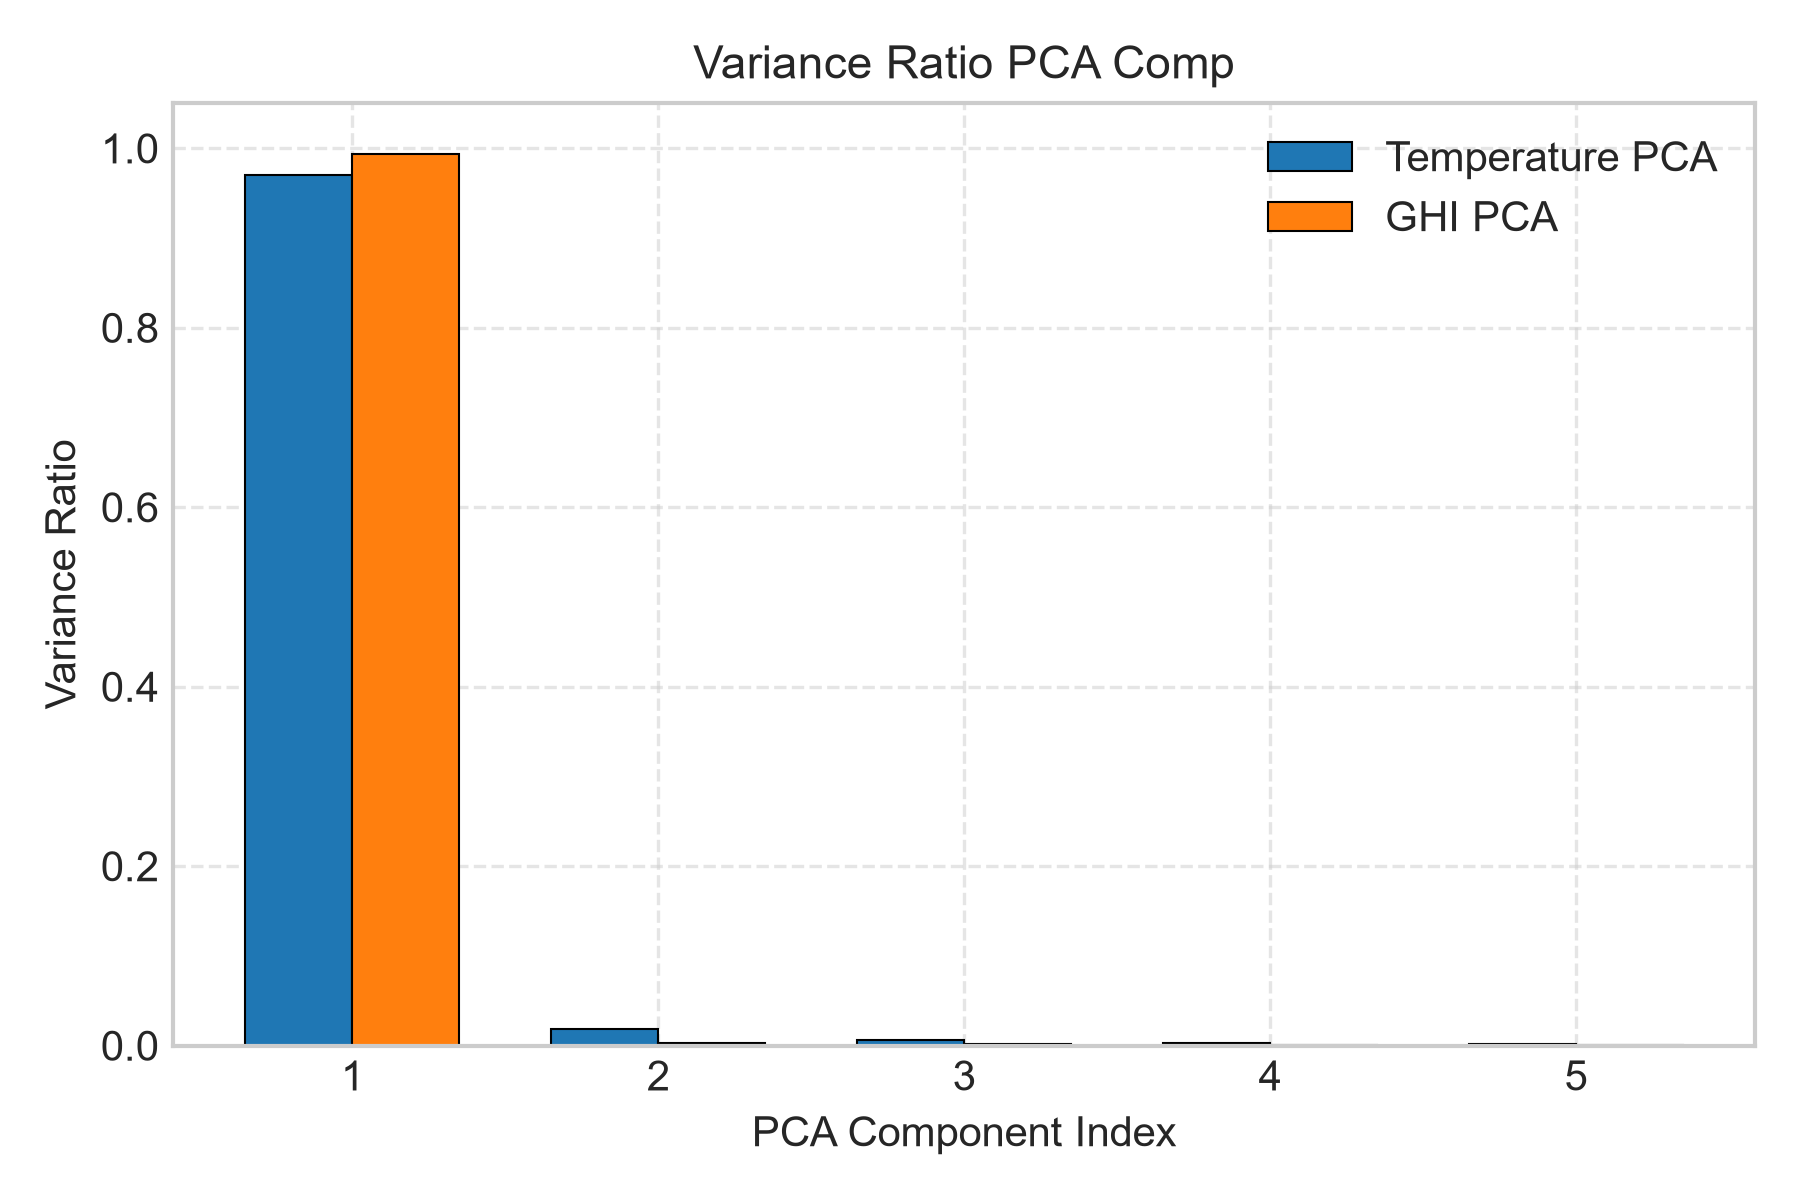
\includegraphics[width=0.75\textwidth]{figures/Figure_3_PCA_Components.png}
    \caption{Tỷ lệ phương sai giải thích của các thành phần chính PCA trên chuỗi Nhiệt độ và Bức xạ mặt trời GHI.}
    \label{fig:pca_components}
\end{figure}

%------------------------------------------------------------------------------
\subsection{Mô-đun 2: Đặc trưng vật lý và chu kỳ liên tục}
\label{subsec:module2}

Kế thừa từ bài báo gốc, mô hình giữ lại các biến trễ động học $\text{PCA\_Temp\_Lag1}$ và $\text{PCA\_GHI\_Lag1}$. Bên cạnh đó, chúng tôi phát triển hai nhóm đặc trưng mới:

\subsubsection{Chỉ số nhu cầu làm mát và sưởi ấm (CDD và HDD)}
\label{subsubsec:hdd_cdd}

Theo nguyên lý truyền nhiệt công trình và tiêu chuẩn ASHRAE~\cite{ashrae2021fundamentals}, lượng nhiệt trao đổi giữa công trình và môi trường tỷ lệ thuận với độ lệch giữa nhiệt độ ngoài trời và nhiệt độ tiện nghi cơ sở $T_{\text{base}} = 18.0^\circ\text{C}$~\cite{quayle1980heating}. Chúng tôi tính:
\begin{align}
    \bar{T}_t &= \frac{1}{5} \sum_{i=1}^5 T_{i, t} \\
    \text{HDD}_t &= \max\left(18.0 - \bar{T}_t, \; 0\right) \\
    \text{CDD}_t &= \max\left(\bar{T}_t - 18.0, \; 0\right)
\end{align}
Hàm $\max(0, \cdot)$ tạo ra tính chất phi tuyến theo ngưỡng: khi thời tiết ôn hòa quanh $18^\circ\text{C}$, cả hai chỉ số đều bằng 0; khi nhiệt độ tăng cao vào mùa hè, chỉ số $\text{CDD}_t$ tăng tỷ lệ thuận và kích hoạt các phản ứng phi tuyến của mô hình cây, giúp nắm bắt chính xác các đợt phụ tải tăng vọt do điều hòa làm mát.

\begin{figure}[htbp]
    \centering
    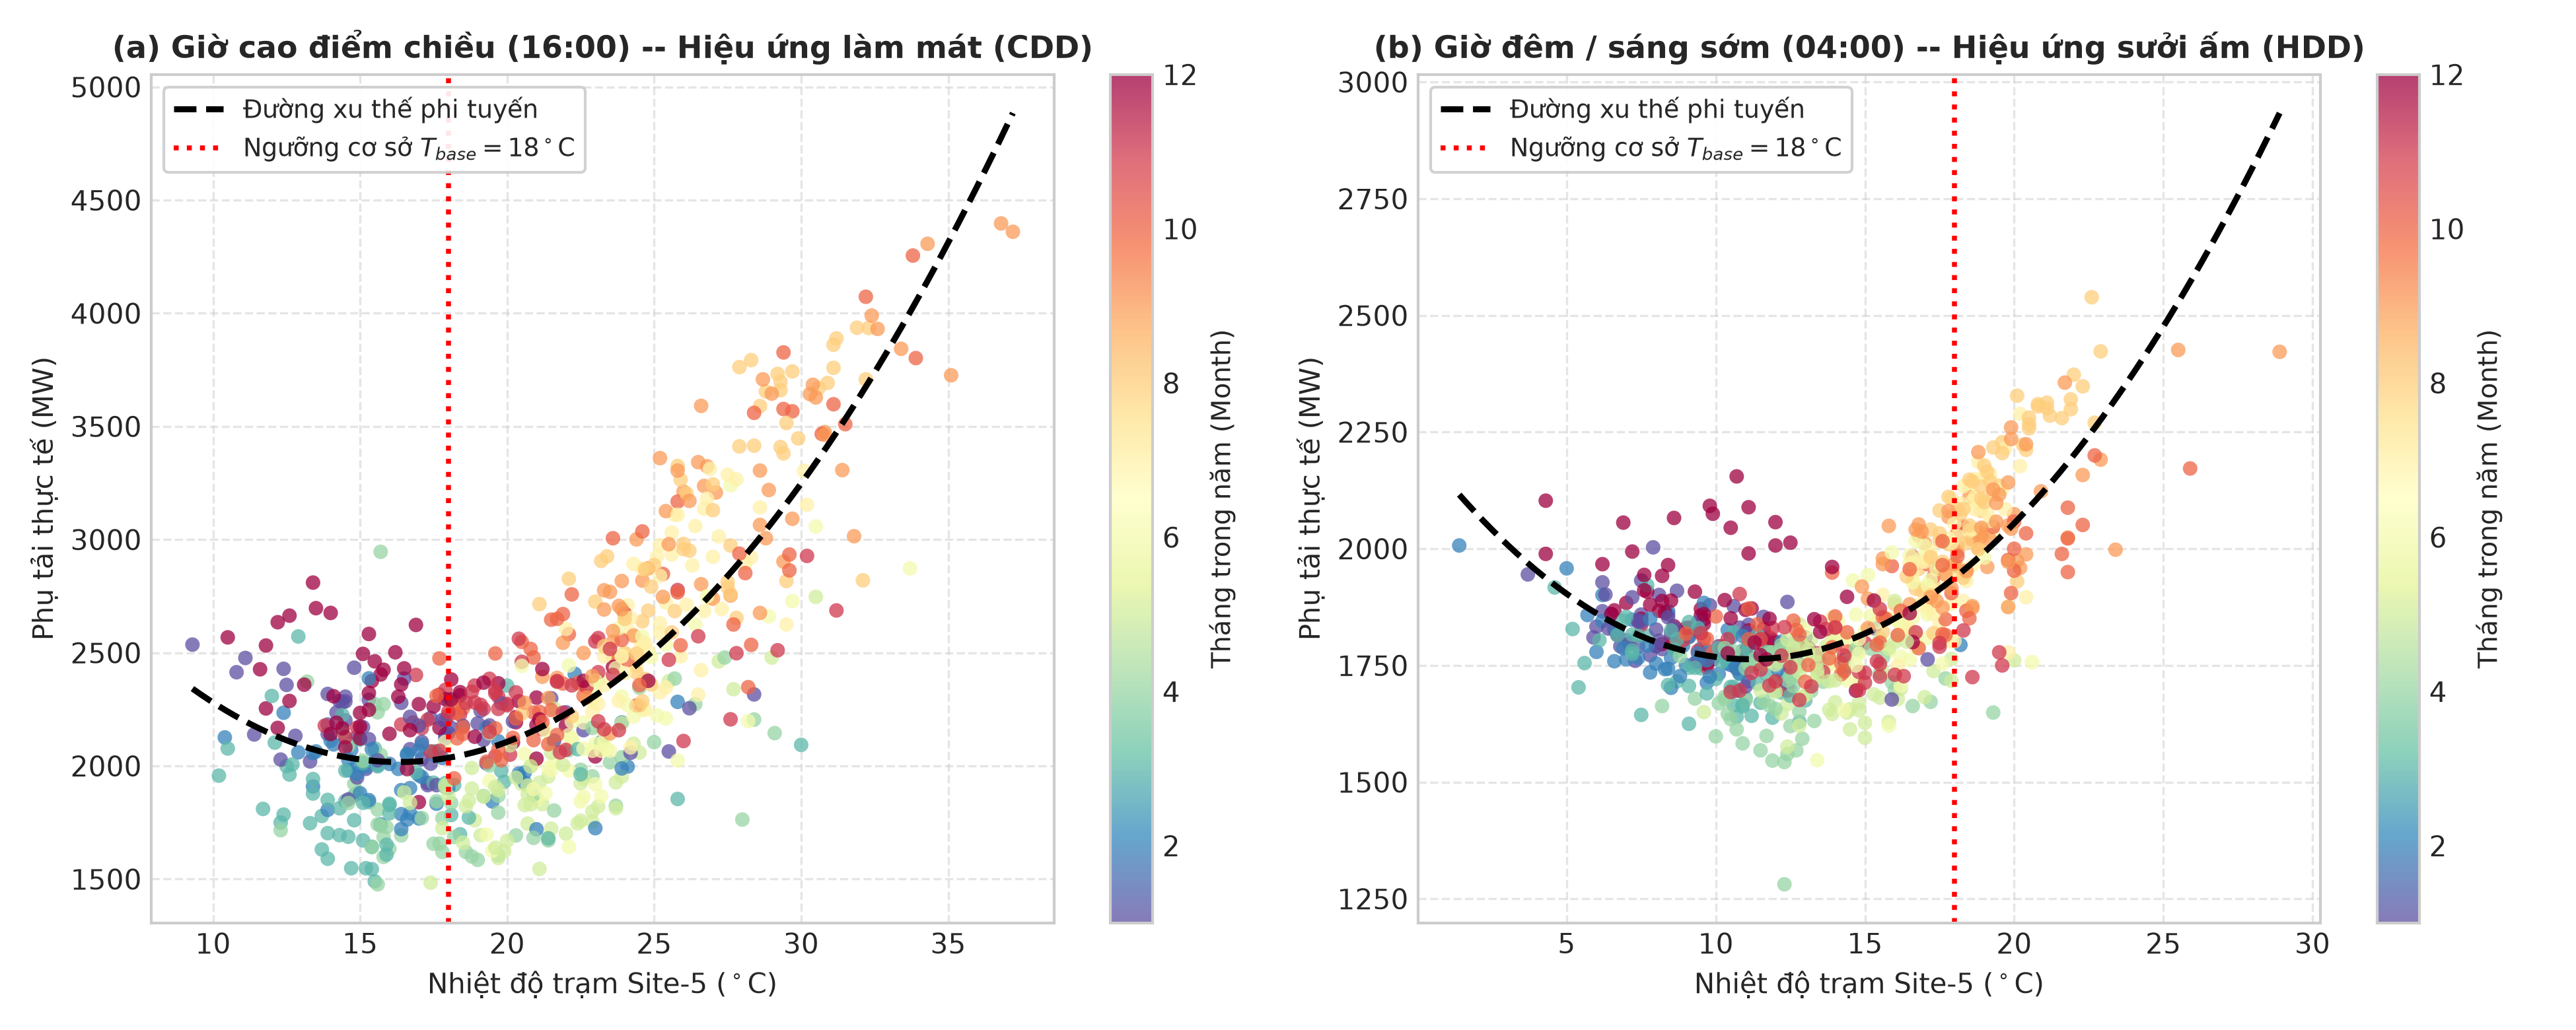
\includegraphics[width=0.96\linewidth]{figures/Figure_Thermal_Response_U_Curve.png}
    \caption{Mối quan hệ phi tuyến hình chữ U giữa nhiệt độ môi trường và phụ tải điện thực tế tại hai khung giờ điển hình: (a) Giờ cao điểm chiều (16:00) minh họa hiệu ứng làm mát bùng nổ (CDD); (b) Giờ rạng sáng (04:00) minh họa hiệu ứng sưởi ấm (HDD). Đường nét đứt màu đỏ biểu diễn ngưỡng tiện nghi nhiệt cơ sở $T_{\text{base}} = 18.0^\circ\text{C}$.}
    \label{fig:thermal_response_u_curve}
\end{figure}

Hình~\ref{fig:thermal_response_u_curve} trực quan hóa dữ liệu thực nghiệm tại hai khung giờ điển hình trong ngày (16:00 chiều và 04:00 sáng). Đồ thị bộc lộ rõ đường cong chữ U kinh điển trong kỹ thuật năng lượng: khi nhiệt độ rơi vào vùng tiện nghi ($15^\circ\text{C}$--$18^\circ\text{C}$), phụ tải điện duy trì ở mức sàn ổn định; khi nhiệt độ giảm sâu dưới $18^\circ\text{C}$, nhu cầu sưởi ấm đẩy phụ tải tăng dần; đặc biệt khi nhiệt độ vượt quá ngưỡng $18^\circ\text{C}$ vào các tháng mùa hè (màu cam và đỏ ở Khung a), phụ tải bùng nổ phi tuyến từ $2.000$~MW lên tới hơn $4.500$~MW do hệ thống điều hòa không khí vận hành hết công suất. Việc đưa CDD và HDD với ngưỡng cơ sở $18^\circ\text{C}$ giúp mô hình học máy tiếp nhận trực tiếp tín hiệu vật lý này thay vì phải tự dò tìm qua các phép chia nhị phân rời rạc của cây quyết định.

\subsubsection{Chuỗi điều hòa Fourier liên tục}
\label{subsubsec:fourier}

Để khắc phục nhược điểm gián đoạn của 12 biến tháng rời rạc, chúng tôi mô hình hóa chu kỳ ngày và chu kỳ năm thông qua các hàm điều hòa Fourier liên tục~\cite{cleveland1990stl, hyndman2018forecasting}:
\begin{align}
    \text{Sin\_Year}_t &= \sin\left(\frac{2\pi \cdot \text{DOY}_t}{365.25}\right), \quad \text{Cos\_Year}_t = \cos\left(\frac{2\pi \cdot \text{DOY}_t}{365.25}\right) \\
    \text{Sin\_Hour}_t &= \sin\left(\frac{2\pi \cdot \text{Hour}_t}{24.0}\right), \quad \text{Cos\_Hour}_t = \cos\left(\frac{2\pi \cdot \text{Hour}_t}{24.0}\right)
\end{align}
trong đó $\text{DOY}_t \in [1, 366]$ là ngày thứ bao nhiêu trong năm (tính theo năm dương lịch thực tế). Các hàm sóng này đảm bảo tính trơn tru liên tục tại thời điểm chuyển giao năm mới và mang lại cơ sở toán học tuần hoàn chặt chẽ.

%------------------------------------------------------------------------------
\subsection{Mô-đun 3: Khám phá hai chế độ vận hành và tính bù trừ sai số}
\label{subsec:module3}

Để chuẩn bị cho mô hình học kết hợp, chúng tôi lựa chọn hai mô hình cơ sở đại diện cho hai trường phái học máy bổ trợ cho nhau:
\begin{enumerate}
    \item \textbf{ElasticNet Regressor (Mô hình tuyến tính với chính quy hóa L1/L2)~\cite{zou2005regularization}:}
    \begin{equation}
        \min_{\mathbf{w}, b} \frac{1}{2N} \sum_{t=1}^N \Big(y_t - \mathbf{w}^T \mathbf{x}_t - b\Big)^2 + \lambda \left[ \alpha \|\mathbf{w}\|_1 + \frac{1 - \alpha}{2} \|\mathbf{w}\|_2^2 \right]
    \end{equation}
    với $\lambda = 0.1, \alpha = 0.5$. Nhờ kết hợp giữa chuẩn $L_1$ (chọn lọc biến thưa) và chuẩn $L_2$ (thu nhỏ hệ số chống cộng tuyến), ElasticNet có phương sai ước lượng thấp, rất ổn định trước nhiễu và phát huy ưu thế tối đa tại vùng phụ tải nền ban đêm.
    \item \textbf{XGBoost Regressor (Mô hình cây quyết định tăng cường gradient)~\cite{chen2016xgboost}:}
    \begin{equation}
        \hat{y}_t = \sum_{k=1}^K f_k(\mathbf{x}_t), \quad f_k \in \mathcal{T}
    \end{equation}
    Mô hình cây sử dụng cấu hình $\text{max\_depth} = 6$ và $200$ cây quyết định ($\text{n\_estimators} = 200$), xuất sắc trong việc phân tách các không gian phụ tải phi tuyến khi nhiệt độ thay đổi mạnh.
\end{enumerate}

Gọi phần dư sai số (\textit{residuals}) dự báo trên tập kiểm tra của hai mô hình là:
\begin{equation}
    e_{\text{enet}, t} = y_t - \hat{y}_{\text{enet}, t}, \quad e_{\text{xgb}, t} = y_t - \hat{y}_{\text{xgb}, t}
\end{equation}
Hệ số tương quan Pearson giữa hai chuỗi phần dư sai số:
\begin{equation}
    r = \frac{\sum_{t=1}^N (e_{\text{enet}, t} - \bar{e}_{\text{enet}})(e_{\text{xgb}, t} - \bar{e}_{\text{xgb}})}{\sqrt{\sum_{t=1}^N (e_{\text{enet}, t} - \bar{e}_{\text{enet}})^2} \sqrt{\sum_{t=1}^N (e_{\text{xgb}, t} - \bar{e}_{\text{xgb}})^2}}
\end{equation}
Giá trị thực nghiệm đo được là \textbf{$r = 0.6131$}. Mức tương quan vừa phải này chứng minh phần dư sai số của hai mô hình có mức độ bù trừ rất cao, là điều kiện lý tưởng để xây dựng mô hình kết hợp (ensemble).

%------------------------------------------------------------------------------
\subsection{Mô-đun 4: Kiến trúc Context-Aware Stacking (CAS)}
\label{subsec:module4}

Trong phương pháp Stacking truyền thống của Wolpert~\cite{wolpert1992stacked}, mô hình tổng hợp (meta-learner) chỉ nhận đầu vào là các giá trị dự báo đơn thuần:
\begin{equation}
    \hat{y}_{\text{traditional}} = g\big(\hat{y}_{\text{enet}}, \hat{y}_{\text{xgb}}\big)
\end{equation}
Mô hình tổng hợp cố định này thiếu thông tin ngữ cảnh môi trường bên ngoài, không thể phân biệt được thời điểm hiện tại đang là giữa trưa nắng nóng hay nửa đêm thanh tĩnh.

Để khắc phục nhược điểm này, kiến trúc \textbf{Context-Aware Stacking (CAS)} mở rộng đầu vào của mô hình tổng hợp LightGBM~\cite{ke2017lightgbm} thành một vector hợp nhất:
\begin{equation}
    \mathbf{z}_t = \Big[ \hat{y}_{\text{enet}, t}^{\text{OOF}}, \; \hat{y}_{\text{xgb}, t}^{\text{OOF}}, \; \mathbf{x}_{\text{context}, t} \Big]^T \in \mathbb{R}^{2 + d_{\text{ctx}}}
\end{equation}
trong đó $\mathbf{x}_{\text{context}, t}$ bao gồm toàn bộ vector ngữ cảnh thời tiết và thời gian: $[\text{Hour}_t, \text{HDD}_t, \text{CDD}_t, \text{Sin\_Year}_t, \text{Cos\_Year}_t, \text{PCA\_Temp}_t, \text{PCA\_GHI}_t, \dots]$.

Để ngăn ngừa triệt để rò rỉ dữ liệu (\textit{data leakage}), vector dự báo của các mô hình cơ sở trong tập huấn luyện được sinh ra thông qua kiểm chứng \textit{Out-Of-Fold} (OOF) bằng kỹ thuật chia tách chuỗi thời gian (\textit{TimeSeriesSplit}) gồm 3 tập con kiểm chứng (\textit{folds}). Mô hình tổng hợp LightGBM được tối ưu hóa siêu tham số bằng thư viện Optuna~\cite{akiba2019optuna} nhằm giảm thiểu RMSE trên các lượt kiểm chứng chéo. Thông qua cơ chế này, mô hình tổng hợp hoạt động như một cơ chế điều phối linh hoạt theo ngữ cảnh: tự động ưu tiên ElasticNet vào ban đêm khi phụ tải phẳng và ổn định, đồng thời chuyển dịch trọng số sang XGBoost khi các đợt nắng nóng đẩy phụ tải lên cao điểm.

%------------------------------------------------------------------------------
\subsection{Cơ sở lý luận lựa chọn phương pháp}
\label{subsec:rationale}

\paragraph{Phù hợp với đặc tính dữ liệu:}
Phụ tải điện theo giờ là chuỗi thời gian phi tuyến, đa trạng thái, với các biến động nhiệt độ phức tạp không thể nắm bắt trọn vẹn chỉ bằng một phương trình tuyến tính đơn thuần. Hiện tượng đa cộng tuyến giữa các trạm quan trắc (VIF lên đến 1055) đòi hỏi bước tiền xử lý PCA bắt buộc. Các chỉ số nhu cầu nhiệt CDD/HDD phản ánh trực tiếp mối quan hệ giữa nhiệt độ và nhu cầu dùng điện làm mát/sưởi ấm, cung cấp thông tin rõ ràng mà mô hình khó có thể tự suy ra từ các biến ngày tháng đơn thuần.

\paragraph{Phù hợp với mục tiêu nghiên cứu:}
Mục tiêu của nghiên cứu là vừa nâng cao độ chính xác dự báo, vừa bảo đảm khả năng giải thích của mô hình. Kiến trúc CAS đáp ứng tốt cả hai yêu cầu: mô hình tổng hợp LightGBM kết hợp với phương pháp SHAP cho phép giải thích cơ chế điều phối; mô hình tuyến tính ElasticNet cung cấp hệ số hồi quy tường minh; và XGBoost phân tách hiệu quả các mối quan hệ phi tuyến phức tạp.

\paragraph{Lợi thế so với các phương pháp hiện có:}
Phương pháp học kết hợp hai tầng theo ngữ cảnh khắc phục hai hạn chế lớn của các phương pháp trước: (a) mô hình tổng hợp truyền thống không nhận biết ngữ cảnh thời gian và thời tiết; (b) biến tháng rời rạc gây bước nhảy đột ngột tại ranh giới chuyển mùa. Chi phí tính toán của CAS hoàn toàn gọn nhẹ: mô hình tổng hợp LightGBM chỉ cần từ 100 đến 250 cây quyết định, toàn bộ quy trình huấn luyện chạy xong trong vài phút trên máy tính cá nhân cho tập dữ liệu 17.520 mốc quan sát.

